\documentclass[10pt]{article}
\usepackage[polish]{babel}
\usepackage[utf8]{inputenc}
\usepackage[T1]{fontenc}
\usepackage{amsmath}
\usepackage{amsfonts}
\usepackage{amssymb}
\usepackage[version=4]{mhchem}
\usepackage{stmaryrd}
\usepackage{graphicx}
\usepackage[export]{adjustbox}
\graphicspath{ {./images/} }

\title{KLASY PO SZKOLE PODSTAWOWEJ }

\author{}
\date{}


\newcommand\Varangle{\mathop{{<\!\!\!\!\!\text{\small)}}\:}\nolimits}

\begin{document}
\maketitle
\begin{enumerate}
  \item Niech \(A B C D\) będzie czworokątem, w którym kąty przy wierzchołkach \(A\) ¡ \(C\) są proste. Mając dane długości \(B C=6, C D=8\) i \(D A=2\), znajdź pole czworokąta ABCD.\\
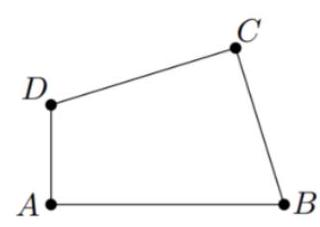
\includegraphics[max width=\textwidth, center]{2024_11_21_64f83780a6f94f658a62g-1(1)}
  \item Dwa kwadraty leżą wewnątrz dużego kwadratu, tak jak pokazano na rysunku. Wyznacz pole kwadratu A, jeśli pole kwadratu B jest równe 48.
  \item W pewnym sklepie sprzedawane są tabliczki mlecznej, białej oraz gorzkiej czekolady, wszystkie po tej samej cenie. Pewnego dnia przychód sklepu ze sprzedaży mlecznej czekolady wyniósł 270, ze\\
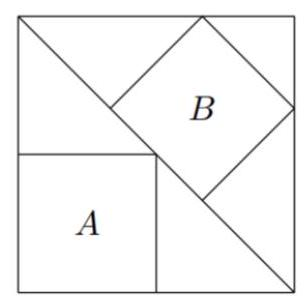
\includegraphics[max width=\textwidth, center]{2024_11_21_64f83780a6f94f658a62g-1}\\
sprzedaży białej - 189, zaś ze sprzedaży gorzkiej - 216. Jaka jest najmniejsza możliwa liczba tabliczek sprzedanych tego dnia w tym sklepie?
\end{enumerate}

\section*{KLASY PO GIMNAZJUM}
\begin{enumerate}
  \item Dane są takie liczby całkowite dodatnie \(x, y, z\), że prawdziwa jest równość:
\end{enumerate}

\[
\frac{x}{y}=\frac{x^{2}+z^{2}}{y^{2}+z^{2}}
\]

Udowodnij, że \(\sqrt{x y}\) jest liczbą całkowitą.\\
2. Dany jest trójkąt prostokątny \(A B C\). Punkt \(D\) jest w nim środkiem przeciwprostokątnej \(A B\). Punkt K i L leżą odpowiednio na odcinkach AD i DB, przy czym KL = CL. Udowodnij, że \(A K \leq 2 D L\).\\
3. Trójkąt \(A B C\) jest różnoboczny. Na boku \(A B\) leżą takie punkty \(K\) i \(L\), że \(A L=A C\) i \(B K=B C\). Prosta równoległa do BC przechodząca przez punkt K i prosta równoległa do \(A C\) przechodząca przez punkt L przecinają się w punkcie S. Wykaż, że \(\Varangle C S K=\Varangle C S L\).


\end{document}